\section{\textbf{{Engenharia de \textit{software}}}}
\label{engenharia-software}

Quando se pensa em desenvolvimento, manutenção, especificação e criação de um \textit{software}, pensa-se também em tecnologias e práticas de gerência de projetos para que a execução da aplicação aconteça de forma organizada, produtiva e com a máxima qualidade possível. Tudo isso esta contido em engenharia de \textit{software}.

Segundo \citeonline{PRESSMAN2016} em seu livro, um \textit{software} bem sucedido é aquele que atende a todos os requisitos do usuário, fica implementado durante um bom tempo, é de fácil manutenção e operabilidade. Por outro lado, um \textit{software} mal sucedido pode acarretar diversos fatos desagradáveis, levando os usuários a insatisfação e ao erro. 

Apesar de gerentes, lideres de projetos e profissionais envolvidos com a área técnica entenderem a necessidade de uma metodologia mais disciplinar no desenvolvimento de \textit{softwares}, existe ainda discursos de como e qual é a melhor metodologia a ser aplicada no projeto. Essa indecisão corre devido a grande demanda de produção que acontece atualmente, principalmente no setor de desenvolvimento de aplicações. Outra coisa que impacta negativamente é que profissionais e empresas começam a desenvolver \textit{softwares} de forma descontrolada mesmo com uma metodologia organizacional aplicada, justamente por não estarem preparados para uma abordagem disciplinar \cite{PRESSMAN2016}. 

Com base nisso, a engenharia de \textit{software} evoluiu rigorosamente, passando de uma simples técnica implementada por um publico relativamente pequeno para uma comunidade que objetiva o planejamento e a organização ates de iniciar qualquer tipo de desenvolvimento.

Sendo assim, em 2001, o engenheiro de \textit{software} Kent Beck juntamente com os principais
desenvolvedores de métodos ágeis, assinaram o “Manifesto para o Desenvolvimento Ágil de Software” \cite{SOMMERVILLE2011}, que tem por iniciativa a seguinte maneira:

\begin{citacao}
“Estamos descobrindo melhores maneiras de desenvolver \textit{softwares}, fazendo-o e ajudando outros a fazê-lo. Através desse trabalho, valorizamos mais:

Indivíduos e interações do que processos e ferramentas;\\
\textit{Software} em funcionamento do que documentação abrangente;\\
Colaboração dos clientes acima de negociação contratual;\\
Respostas a mudanças acima de seguir um plano;\\
Ou seja, embora itens à direita sejam importantes, valorizamos mais os que estão à esquerda.\cite{SOMMERVILLE2011}"

\end{citacao}

\subsection{{Desenvolvimento ágil de \textit{software}}}

Quando se pensa em desenvolvimento de \textit{software}, deve-se reconhecer que o processo é bem instável e com baixa previsibilidade, se tornando algo complicado de estabelecer métricas a serem seguidas. Vários pontos de interferência pode intervir para que um \textit{software} não possa ser desenvolvido da maneira correta, como por exemplo uma equipe de trabalho desestruturada, nos quais os integrantes não possuem uma boa convivência entre si, ou uma metodologia de desenvolvimento sem uma linha cronológica a ser seguida. Reconhecer que este é um grande desafio é algo sensato de se fazer. No entanto existem mecanismos de correção para melhorar o processo de desenvolvimento.

A metodologia ágil surgiu para organizar esses processos de desenvolvimento de \textit{software}, elaborando uma padronização nos projetos para que seja possível otimizar os fluxos de trabalho e melhoras a produtividade do projeto. Segundo \citeonline{SOARES2004}, a principal característica da metodologia ágil e que ela pode ser adaptada, ao invés de ser preditiva. Ou seja, se ocorrer algum problema no decorrer do desenvolvimento, a própria metodologia é flexível o bastante para contornar a situação e prosseguir com o desenvolvimento do projeto. Portanto, uma empresa pode facilmente criar a sua própria metodologia de trabalho, seguindo a sua experiência empresarial, analisando os seus acertos e erros para elaborar um procedimento que se adéqua as suas necessidades. 

\citeonline{SOARES2004} continua exemplificando que a metodologia ágil trabalha com constantes \textit{feedbacks} e reuniões, nas quais permitem aos membros da equipe expor as facilidades e dificuldades de suas tarefas, bem como o seu status de desenvolvimento. A partir destes \textit{feedbacks}, o gestor pode traçar a melhor maneira de organizar a equipe para que os membros com maior experiência deem apoio nas dificuldades apresentadas pelos outros integrantes da equipe. Outro grande motivo expressado no contexto é o fato ocorrer entregas constantes de partes operacionais do software. Desta maneira, o usuário final do software pode ter uma prévia de como o sistema está sendo desenvolvido, bem como suas funcionalidades e \textit{design}, podendo solicitar alguma possível alteração ou identificar algum problema antes da implantação oficial dos modulos.

\subsubsection{\textit{Kanban}}

O \textit{Kanban} é um método organizacional de desenvolvimento de software que permite a interação de várias áreas e membros do projeto por meio de cartões que contém o progresso de cada atividade. Cada cartão contém uma instrução a ser seguida pela área ou pelo integrante no qual foi designado para a atividade. Sendo assim, seu principal foco e fornecer um trabalho progressivo, apresentando as evoluções e dificuldades de forma clara e transparente, favorecendo uma cultura de melhoria contínua \cite{KANBAN2014}.

Portanto, a ferramenta \textit{Kanban} tem um grande potencial em trabalho conjunto para a finalização de um item em específico, justamente para que não ocorra nenhum gargalo na entrega de um item essencial para o trabalho do integrante ou da área seguinte. Outra grande característica é evitar ou diminuir o índice de trabalhos repetitivos que, por um eventual descuido, possa acontecer de desenvolvedores realizarem a mesma codificação de uma mesma função ou \textit{API - Application Programming Interface} (Interface de Programação de Aplicações), por exemplo.

A abordagem \textit{Kanban} foi criada pelo vice presidente da \textit{Toyota Motor Company}, o Sr. Taiichi Ohno, no qual teve como principal objetivo o aumento do valor agregado entregue nas atividades de cada colaborador de sua equipe. Com este pensamento,  Ohno concluiu que as pilhas de materiais estocados e as filas de espera eram equivalentes à um “dinheiro parado” que a empresa \textit{Toyota} estava desperdiçando. Portando,   Ohno uniu os princípios do método \textit{just in time} (determina que tudo deve ser feito na hora exata)  juntamente com o \textit{Jidoka} (determina que corrigir o problema em si não é o bastante, e sim corrigir a origem do problema) para elaborar um método mais aprimorado de organização dentro da empresa \textit{Toyota}, denominado \textit{Kanban} \cite{TOYOTA1977}.

Devido à sua simplicidade, fácil implantação, entendimento e manipulação, atualmente a abordagem \textit{Kanban} é utilizada em diversas empresas para realizar o controle de desempenho de diversas área. A \autoref{fig_kanban} demonstra um exemplo clássico de uma abordagem \textit{Kanban}.

\begin{figure}[h]
	\caption{\label{fig_kanban}Exemplo de uma abordagem \textit{Kanban}.}
	\begin{center}
		\resizebox{1\linewidth}{!}{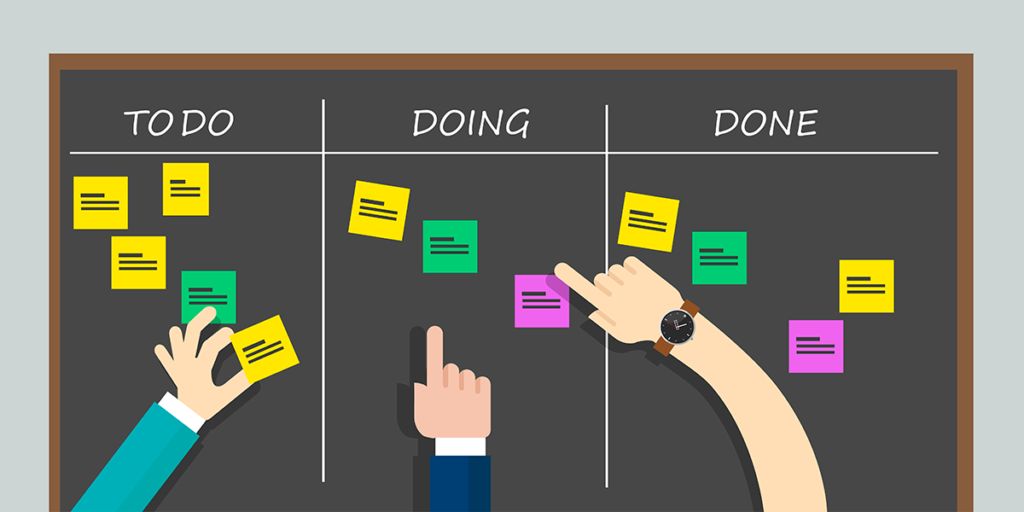
\includegraphics{4-Conteudo-Bibliografico/3-Engenharia-Software/kanban.png}}
	\end{center}
	\centering \legend{Disponível em: https://novida.com.br/blog/kanban/}
\end{figure}

\subsubsection{\textit{Trello}}

O \textit{Trello} é uma ferramenta de gerenciamento de projetos que tem por finalidade auxiliar os lideres de projetos a organizar da melhor forma o fluxo de tarefas relacionadas ao seu trabalho. Utilizando o método \textit{Kanban}, todas as atividades disponibilizadas no \textit{Trello} são exibidas em um único ambiente de trabalho visível por todos os membros da equipe que foram adicionados a ele. As organizações das atividades são feitas através de \textit{cards} (cartões), onde cada membro fica responsável por exercer a atividade que lhe foi designada. O \textit{Trello } possui uma interface bastante amigável e simples de entender \cite{TRELLO2017}. 

Por ser uma aplicação \textit{Web}, o \textit{Trello} necessita de uma conexão com a internet para que os trabalhos possam ser compartilhados e disponibilizados para toda a equipe. A aplicação disponibiliza grandes possibilidades de organização, como por exemplo a criação de atividades distintas dentro de um mesmo projeto, classificação das atividades com rótulo de cores (urgente, não urgente, pouco urgente, descartar, etc), definir a situação de cada atividade (concluída, a fazer, fazendo, etc), dentre outras. Outra grande utilidade que o \textit{Trello} disponibiliza são as notificações por e-mail, que notifica a todos os membros a situação de suas atividades dentro do projeto, bem como seu \textit{status} e prazo.